\documentclass[ngerman]{dis-template-add}


\renewcommand{\Aufgabenblatt}{1}
\renewcommand{\Ausgabedatum}{28. April 2020}
\renewcommand{\Abgabedatum}{8. Mai 2020}
\renewcommand{\Gruppe}{Simon Weidmann, Aram Yesildeniz}
\renewcommand{\STiNEGruppe}{14}


\begin{document}


\section*{1.2 DB-Schema}

\subsection*{Tables}

=> Horizontal Partitioning

\begin{center}

Estate Agent \\
\begin{tabular}{ c | c | c | c }
 \soliduline{Login} & Name & Address & Password \\
 \hline
  & & & \\
\end{tabular}

Estate \\
\begin{tabular}{ c | c | c | c | c | c | c }
 \soliduline{ID} & City & Postal Code & Street & Street Number & Square Area & \dashuline{Manager = EsateAgent.Login} \\
 \hline
  & & & & & & \\
\end{tabular}

Apartment \\
\begin{tabular}{ c | c | c | c | c | c | c | c | c | c | c | c }
 \soliduline{ID} & City & PC & Str. & Str.Nr. & SA & Floor & Rent & Rooms & Balcony & Kitchen & \dashuline{Manager = EsateAgent.Login} \\
 \hline
  & & & & & & & & & & &  \\
\end{tabular}

House \\
\begin{tabular}{ c | c | c | c | c | c | c | c | c | c }
 \soliduline{ID} & City & PC & Str. & Str.Nr. & SA & Floors & Price & Garden & \dashuline{Manager = EsateAgent.Login} \\
 \hline
  & & & & & & & & & \\
\end{tabular}

Person \\
\begin{tabular}{ c | c | c | c }
 \soliduline{ID} & First Name & Name & Address \\
 \hline
  & & & \\
\end{tabular}

Contract \\
\begin{tabular}{ c | c | c  }
 \soliduline{Contract No.} & Date & Place\\
 \hline
  & & \\
\end{tabular}
  
Tenancy Contract  \\
\begin{tabular}{ c | c | c  | c | c  | c | c | c  }
 \soliduline{Con.No.} & Date & Place & Start D. & Dur. & Add.Costs & \dashuline{Person.ID} & \dashuline{Apartment.ID} \\
 \hline
  & & & & & & & \\
\end{tabular}

Purchase Contract  \\
\begin{tabular}{ c | c | c  | c | c  | c | c  }
 \soliduline{Con.No.} & Date & Place & No.of.Install. & Intrest Rate & \dashuline{Person.ID} & \dashuline{House.ID} \\
 \hline
  & & & & & & \\
\end{tabular}

\end{center}


%\begin{RMSchma}
%Person(\soliduline{PID}, Name, Vorname, \dashuline{(HaustierName, HaustierRasse) $\rightarrow$ (Haustier.Name, Haustier.Rasse)})
%Haustier(\soliduline{Name, Rasse}, \dashuline{Herrchen $\rightarrow$ Person.PID})
%\end{RMSchma}




%\section{Beispiel für Ausdruck der Relationenalgebra}

%\begin{align*}
% &\umbenennung{Rasse}{Sorte}(\projektion{Rasse, Geschlecht}((Wolf\verbund{Wolf.WID=Haustier.HID} (\selektion{Name=\wert{Hasso}}Haustiere)) \natverbund Person))
%\\  &=\{ \wert{Steppenwolf}, \wert{m} \}
%\end{align*}


\subsection*{SQL Scripts}

\subsection*{Create Database}

\begin{verbatim}
CREATE DATABASE dis
    WITH 
    OWNER = postgres
    ENCODING = 'UTF8'
    CONNECTION LIMIT = -1;
\end{verbatim}


\subsection*{Create Tables}

\begin{verbatim}
CREATE TABLE public.estate_agent
(
    agent_login text,
    agent_name text,
    agent_address text,
    agent_password text,
    PRIMARY KEY (agent_login)
);

ALTER TABLE public.estate_agent
    OWNER to postgres;
    

CREATE TABLE public.estate
(
    estate_id serial,
    city text,
    postal_code integer,
    street text,
    street_number text,
    square_area integer,
    manager text,
    PRIMARY KEY (estate_id),
    CONSTRAINT manager FOREIGN KEY (manager)
        REFERENCES public.estate_agent (agent_login) MATCH SIMPLE
        ON UPDATE NO ACTION
        ON DELETE NO ACTION
        NOT VALID
);

ALTER TABLE public.estate
    OWNER to postgres;


CREATE TABLE public.apartment
(
    floor integer,
    rent text,
    rooms text,
    balcony boolean,
    kitchen boolean,
    CONSTRAINT apartment_pkey PRIMARY KEY (estate_id),
    CONSTRAINT manager FOREIGN KEY (manager)
        REFERENCES public.estate_agent (agent_login) MATCH SIMPLE
        ON UPDATE NO ACTION
        ON DELETE NO ACTION
        NOT VALID
)
    INHERITS (public.estate);

ALTER TABLE public.apartment
    OWNER to postgres;


CREATE TABLE public.house
(
    floors integer,
    price text,
    garden boolean,
    CONSTRAINT house_pkey PRIMARY KEY (estate_id),
    CONSTRAINT manager FOREIGN KEY (manager)
        REFERENCES public.estate_agent (agent_login) MATCH SIMPLE
        ON UPDATE NO ACTION
        ON DELETE NO ACTION
)
    INHERITS (public.estate)
TABLESPACE pg_default;

ALTER TABLE public.house
    OWNER to postgres;


CREATE TABLE public.person
(
    id serial,
    first_name text,
    last_name text,
    address text,
    PRIMARY KEY (id)
);

ALTER TABLE public.person
    OWNER to postgres;


CREATE TABLE public.contract
(
    contract_number serial,
    contract_date date,
    place text,
    PRIMARY KEY (contract_number)
);

ALTER TABLE public.contract
    OWNER to postgres;


CREATE TABLE public.tenancy_contract
(
    start_date date,
    duration text,
    additional_costs text,
    person_id integer,
    apartment_id integer,
    CONSTRAINT tenancy_contract_pkey PRIMARY KEY (contract_number),
    CONSTRAINT person_id FOREIGN KEY (person_id)
        REFERENCES public.person (id) MATCH SIMPLE
        ON UPDATE NO ACTION
        ON DELETE NO ACTION
        NOT VALID,
    CONSTRAINT apartment_id FOREIGN KEY (apartment_id)
        REFERENCES public.apartment (estate_id) MATCH SIMPLE
        ON UPDATE NO ACTION
        ON DELETE NO ACTION
        NOT VALID
)
    INHERITS (public.contract);

ALTER TABLE public.tenancy_contract
    OWNER to postgres;


CREATE TABLE public.purchase_contract
(
    installment_amount text,
    intrest_rate text,
    person_id integer,
    house_id integer,
    CONSTRAINT purchase_contract_pkey PRIMARY KEY (contract_number),
    CONSTRAINT person_id FOREIGN KEY (person_id)
        REFERENCES public.person (id) MATCH SIMPLE
        ON UPDATE NO ACTION
        ON DELETE NO ACTION
        NOT VALID,
    CONSTRAINT house_id FOREIGN KEY (house_id)
        REFERENCES public.house (estate_id) MATCH SIMPLE
        ON UPDATE NO ACTION
        ON DELETE NO ACTION
        NOT VALID
)
    INHERITS (public.contract);

ALTER TABLE public.purchase_contract
    OWNER to postgres;
\end{verbatim}


\subsection*{Insert Estate Agent}

\begin{verbatim}
INSERT INTO public.estate_agent(
    agent_login, agent_name, agent_address, agent_password)
    VALUES ('testagent', 'testname', 'testaddress', 'testpassword');
\end{verbatim}



\section*{1.3 Java Application - Questions}

\textit{Create an apartment, an estate agent and a tenancy contract with your java application. Validate that they are in the database (e.g. by using a screenshot of application and database).}

\subsection*{Create Estate Agent}
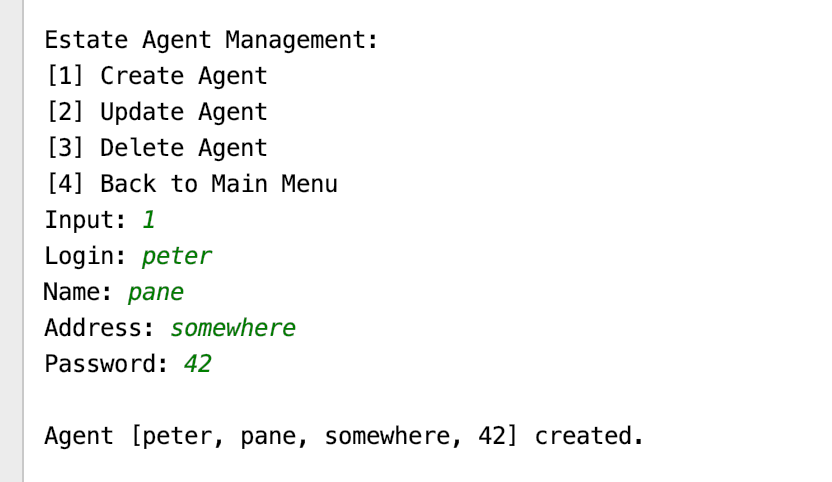
\includegraphics[scale=.5]{agent_app} \\
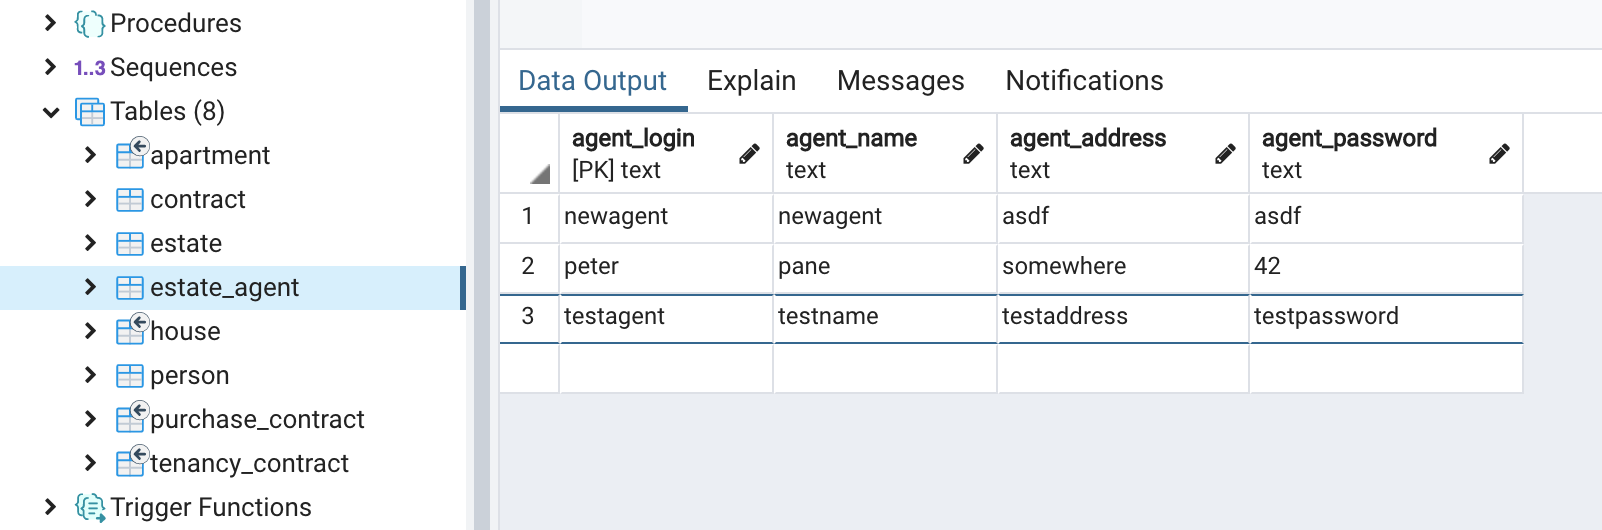
\includegraphics[scale=.5]{agent_db}

\subsection*{Create Apartment}
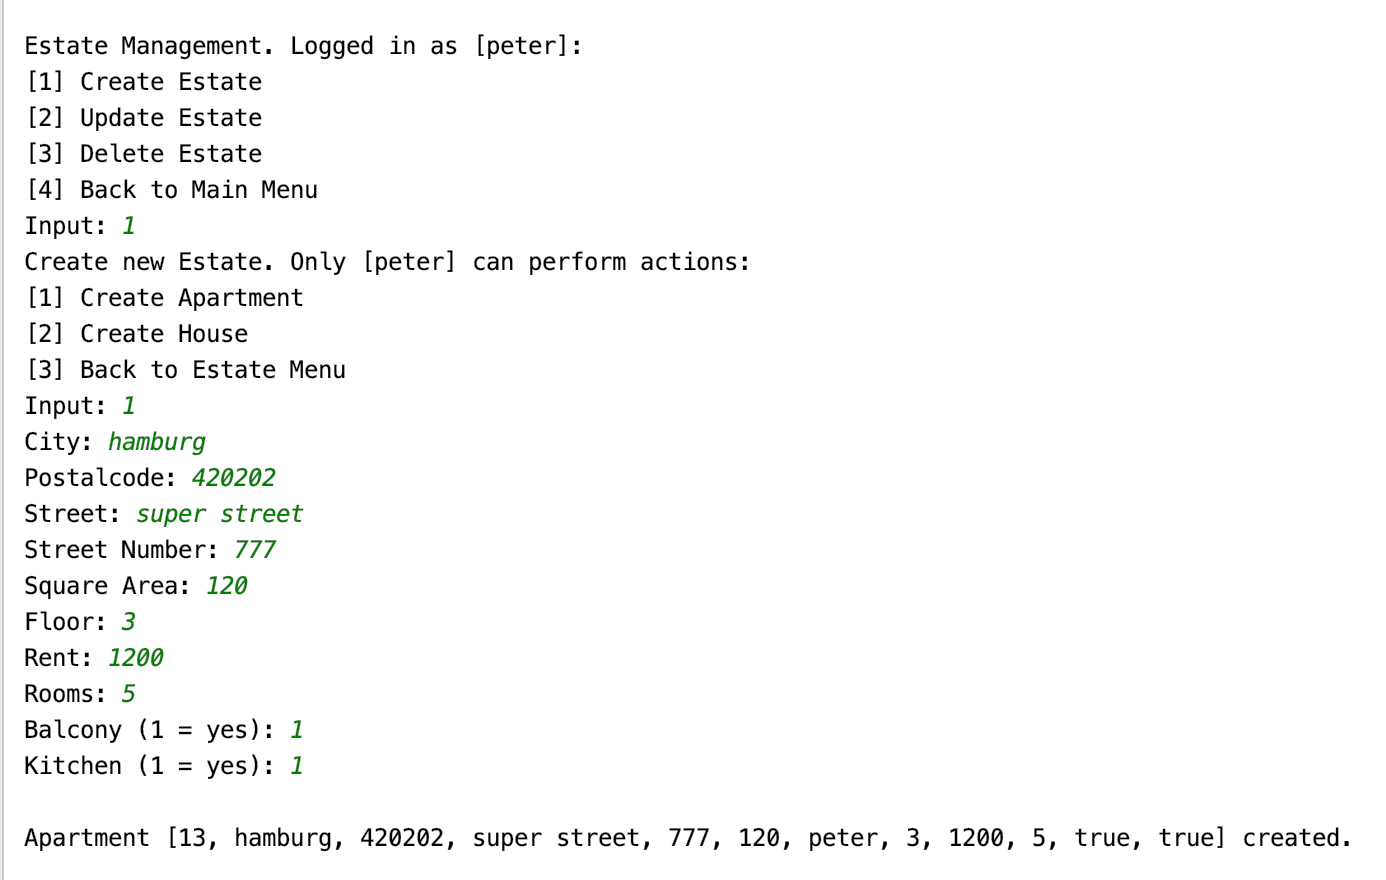
\includegraphics[scale=.5]{estate_app} \\
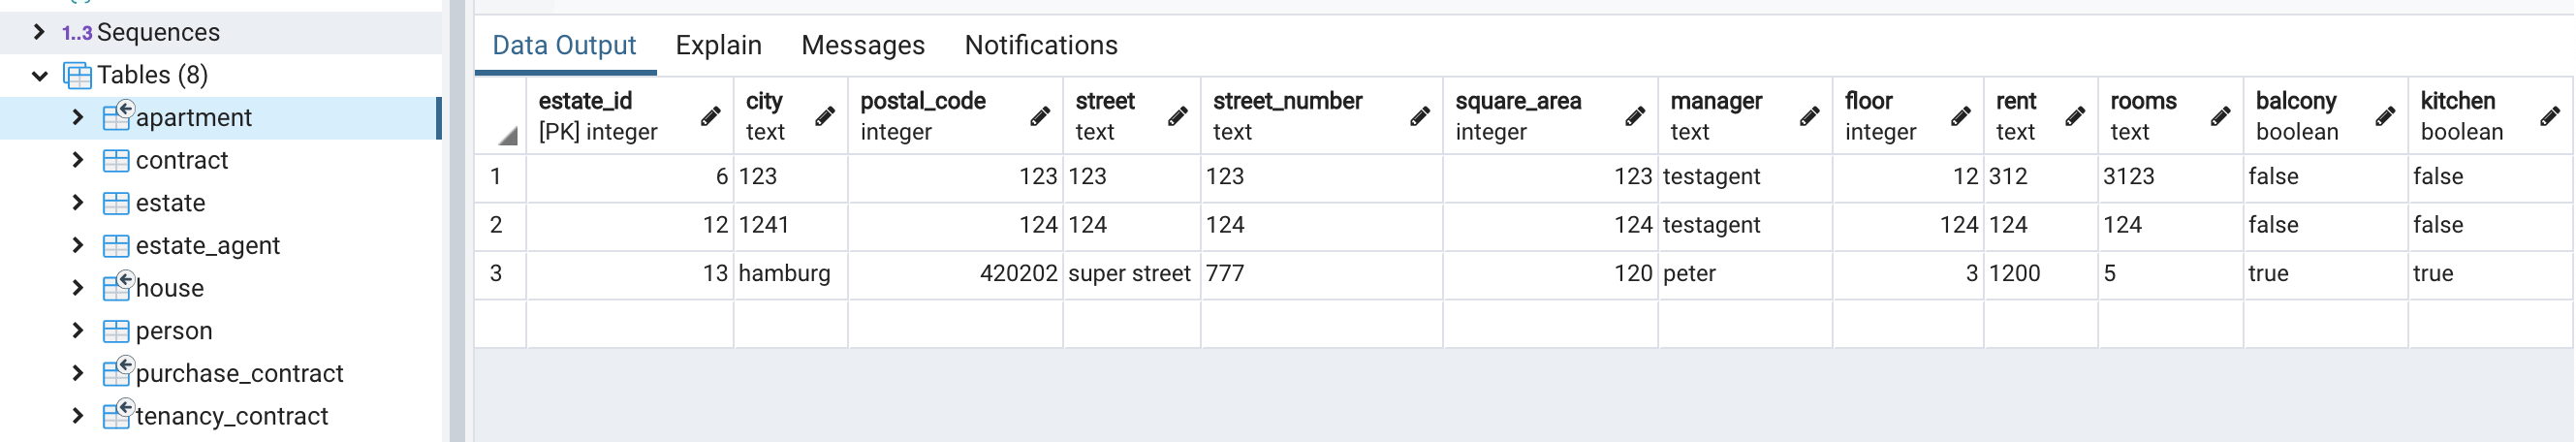
\includegraphics[scale=.3]{estate_db}

\subsection*{Create Tenancy Contract}
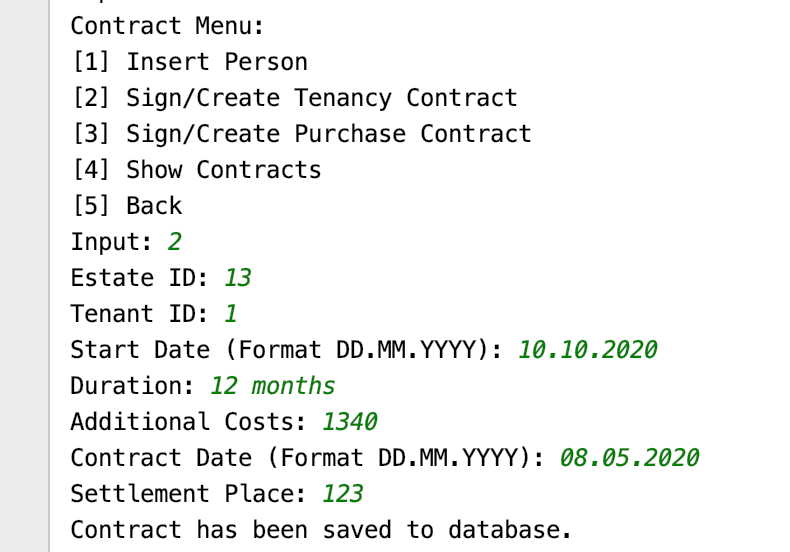
\includegraphics[scale=.5]{contract_app} \\
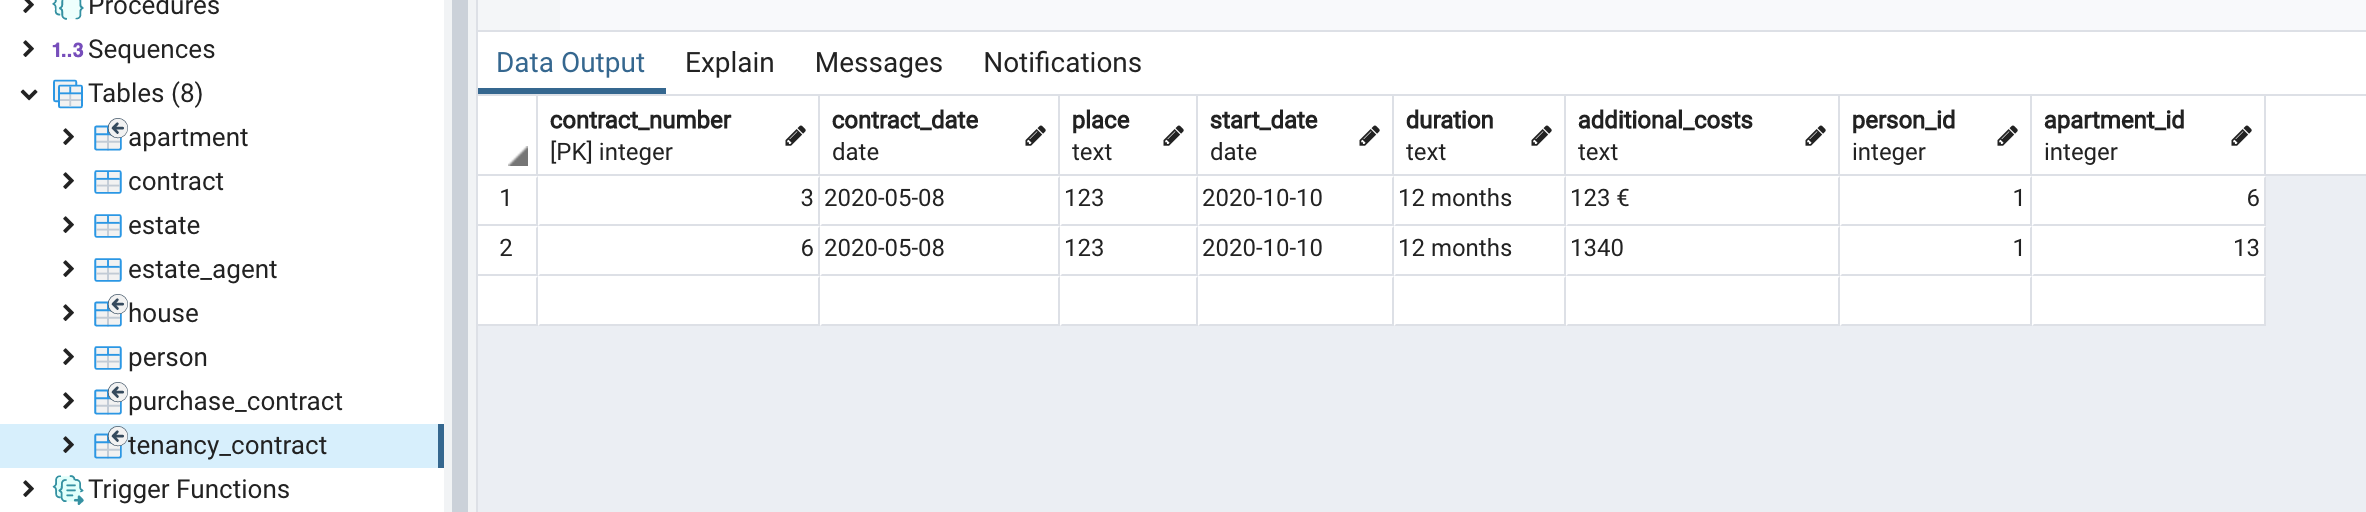
\includegraphics[scale=.4]{contract_db} \\ \\


\textit{Create a contract with a non-existing estate. Does it work? Why/Why not?
} \\
No it does not work. The foreign key `apartment-id' in the tenancy contract table needs to be valid. If the entered id is not existing in the corresponding estate table, an exception will be thrown: \\
ERROR: insert or update on table tenancy-contract violates foreign key constraint person-id \\
Detail: Key (person-id)=(123) is not present in table person.

\textit{Which inheritance model did you choose and why?
} \\
Horizontal: Postgresql offers the INHERITS keyword, which enables horizontal partitioning. Therefore we used this keyword because it is intuitive to use easy to implement.

\textit{Create an apartment, and let your application crash between inserting the estate information and inserting the apartment information. What is the effect on your database state?
} \\
Since it is only possible to create an apartment or house in one go, this use case will not happen.
If the application crashes while the user inserts information for the estate he wants to create, the record will not be saved.


\end{document}